\chapter{Solution Approach}
\label{ch:Solution Approach}
%\section{Survey EEG based Authentication Systems}

This study aims to develop a benchmarking suite on EEG-based authentication
systems for a larger set of participants (N>100) using various open medical-grade EEG
datasets. The performance and robustness of the different authentication algorithms will be compared with appropriate metrics to determine which algorithm is most effective and on which dataset. This section comprehensively describes the tasks performed to compare the performance of different brainwave authentication algorithms.
on open EEG datasets.

\section{Survey Open Datasets}
\label{sec:Solution Approach:Survey Open Datasets}
Creating an efficient and robust EEG benchmarking framework involves collecting high-quality EEG datasets, which is essential since the quality of datasets can significantly influence the overall effectiveness of the framework. The following issues can arise if poor-quality datasets are used for developing the benchmarking framework: 
\begin{enumerate}
\item \textbf{Random Classification}: Noise in the EEG data can obscure the model from identifying the meaningful brain data and random noise. It could lead the model randomly classify the users based on their brain data.
    
\item \textbf{Erroneous or Biased Results}: The imbalance in the participant's population in the datasets may lead to overestimating the evaluation metrics such as accuracy \cite{sugrim_robust_metrics}. Additionally, skewed datasets introduce biases into the system, so the results generated by those authentication systems cannot be trusted.    

\item \textbf{Increased Pre-Processing Time}: Most of the data cleaning is done during the pre-processing stage, and considering that the bad quality datasets also have a low signal-to-noise ratio (SNR), the researchers often spend considerable amount of time, handling the noisy data.

\item \textbf{Overfitting or Underfitting}: Bad quality datasets can lead to overfitting or underftitting while creating the machine learning models. Overfitting occurs when the model is too complex that it starts learning from the noise, and underfitting arises when the model is too simple to understand the intricate patterns in the data. Both of these situations may result in inaccurate predictions. 

\item \textbf{Limited Reproducibility}: If the datasets are of bad quality, the other researchers would not be able to reproduce the results, questioning the reliability of the initial research. 
\end{enumerate}

Although consumer devices offer simplicity and are more user-friendly than traditional EEG devices, their EEG data have lower SNR than EEG devices. And considering the potential pitfalls associated with utilizing low SNR datasets, we focus on high-quality medical-grade EEG datasets for our study. Open datasets vary across the EEG headsets, the number of electrodes (channels), stimuli tasks, EEG paradigms, physical setup, and file format. As a result, researchers have traditionally recorded a new dataset or used one of the few well-known datasets when they have to validate a new approach \cite{moabb}. However, recording a new medical-grade EEG dataset can be an intricate task as it requires experts' assistance to set up the devices and correctly monitor the participant's brain activity. Therefore, our study primarily focuses on harnessing publicly available high-quality EEG datasets as the first step.
\smallskip

Considering that ERPs have a reasonably good SNR, less susceptibility to background perturbations \cite{armstrong2015brainprint}, and can assess instantaneous reactions to short stimuli \cite{zhang2021review}, we propose to focus on the comparison of different algorithms based on ERP paradigms like P300 and N400 which can fill the gaps left by other data acquisition protocols and provides a more robust authentication mechanism. P300 is a positive deflection in voltage that reaches its peak at 300 milliseconds (ms) following exposure to a specific stimulus and is usually triggered using the "oddball" paradigm, in which a subject detects an occasional or rare stimulus in a regular train of standard stimuli \cite{picton1992p300}—for example, encountering a picture of an animal (a rare stimulus) in a series of images, targeting human celebrities (standard stimuli). On the other hand, N400 is a negative deflection that peaks around 400 ms after the presentation of a stimulus, and N400 responses are associated with stimuli connected to semantic processing, such as language processing \cite{arias2021inexpensive}. As a result, we decided to exclusively survey and concentrate on the open datasets based on ERP paradigms like P300 and N400 on the internet.  
\smallskip

Collecting quality EEG datasets was tedious since most researchers in the EEG domain do not make their dataset public because of privacy and confidentiality issues. Nevertheless, despite these obstacles, our assiduous search yielded more than 40 datasets, procured from websites known for providing repositories for high-quality EEG datasets, such as \textbf{OpenBCI} \footnote{\url{https://openbci.com/community/publicly-available-eeg-datasets/}}, \textbf{Zenodo} \footnote{\url{https://zenodo.org/}}, \textbf{MOABB} \footnote{\url{http://moabb.neurotechx.com/docs/datasets.html}}, \textbf{Dryad} \footnote{\url{https://datadryad.org/stash}}, \textbf{OSF} \footnote{\url{https://osf.io/}} and \textbf{Figshare} \footnote{\url{https://figshare.com/}}. Table \autoref{tab:Table 1} and \autoref{tab:Table 2} list some of the publicly available P300 and N400 datasets that we reviewed during our study, organized chronologically by the year of their release. Four datasets \cite{bi2015a, cogbci, kappenman2021erp, mantegna2019distinguishing} were selected for our research, based on the ERP and the other criteria: 1) an ERP paradigm such as P300 or N400 2) raw data available 3) implementation code available 4) Multi samples per subject available 6) Number of subjects (N>=25). We chose the second condition to apply the standardized pre-processing, feature extraction, and authentication steps across all datasets. This uniform process is essential to evaluate their performance under similar experimental conditions, which is impossible without access to unprocessed raw data. As a result, we discarded datasets from our study which only provided pre-processed data. Additionally, we did not want to utilize datasets where subjects provide a single sample because a single brain sample cannot capture the EEG variability across different instances of the same subject. Consequently, we applied the condition to include only the datasets with multiple samples per subject. In the subsequent sections, we provide a concise overview of the datasets that were excluded and included in our study, respectively. The datasets that were excluded from our study had the potential to be included, but ultimately were not incorporated due to the aforementioned conditions \cite{}.  
% \begin{itemize}
%     \item \textbf{Lee et al.} \cite{lee2019eeg}: 
% \end{itemize}

\begin{table}[ht]
\caption{Publicly available ERP datasets based on P300 (oddball) paradigm}
\label{tab:Table 1}

\resizebox{\textwidth}{!}
    {
\begin{tabular}{c|cccccccc}

\hline

%Table column names
\rule{0pt}{25pt} \textbf{Dataset} & \textbf{Year} & \textbf{$\#$Subjects} & \textbf{EEG Device} & \textbf{$\#$Channels} & \textbf{Sampling Rate} & \textbf{$\#$Sessions} & \textbf{EEG task}\\
%\hline
%Data Acquistation Row
\hline
\rowcolor{Gray}
\rule{0pt}{25pt} \textbf{BrainInvaders12 \cite{van2019building}} & 2012 & 25 & NeXus-32 & 16 & 128 Hz & 1 & Visual Stimuli \\

\rule{0pt}{25pt} \textbf{BrainInvaders13a \cite{vaineau2019brain}} & 2013 & 24 & g.GAMMAcap  & 16 & 512 Hz & 1 & Visual Stimuli\\

\rowcolor{Gray}
\rule{0pt}{25pt} \textbf{BrainInvaders14a \cite{bi2014a}} & 2014 & 64 & g.Sahara & 16 & 512 Hz & 1 & Visual Stimuli\\

%ERP Devices Row
\rule{0pt}{25pt}\textbf{BrainInvaders14b \cite{bi2014b}} & 2014  & 37 & g.GAMMAcap & 32 & 512 Hz & 1 & Visual Stimuli\\

\rowcolor{Gray}
\rule{0pt}{25pt} \textbf{Gao et al. \cite{gao2014novel}} & 2014 & 30 & Neuroscan & 12 & 500 Hz & 1 & Visual Stimuli\\

\rule{0pt}{25pt}\textbf{BrainInvaders15a \cite{bi2015a}} & 2015 & 43 & g.GAMMAcap & 32 & 512 Hz & 1 & Visual Stimuli\\

\rowcolor{Gray}
\rule{0pt}{25pt}\textbf{BrainInvaders15b \cite{bi2015b}} & 2015 & 44 & g.GAMMAcap & 32 & 512 Hz & 1 & Visual Stimuli\\

\rule{0pt}{25pt}\textbf{Mouček et al. \cite{mouvcek2017event}} & 2017 & 250 & BrainVision & 3 & n.a. & 1 & Visual Stimuli\\

\rowcolor{Gray}
\rule{0pt}{25pt}\textbf{Hubner et al. \cite{hubner2017learning}} & 2017 & 13 & \vtop{\hbox{\strut BrainAmp DC, }\hbox{\strut Brain Products}} & 31 & 1000 Hz & 1 & \vtop{\hbox{\strut Visual Stimuli}\hbox{\strut Auditory Stimuli}}\\

\rule{0pt}{25pt}\textbf{Sosulski and Tangermann \cite{sosulski2019spatial}} & 2019  & 13 & \vtop{\hbox{\strut BrainAmp, }\hbox{\strut EasyCap}} & 31 & 1000 Hz & 1 & Visual Stimuli\\

\rowcolor{Gray}
\rule{0pt}{25pt}\textbf{Lee et al. \cite{lee2019eeg}} & 2019  & 54 & BrainAmp & 62 & 1000 Hz & 2 & Visual Stimuli\\

\rule{0pt}{25pt}\textbf{Simões et al. \cite{simoes2020bciaut}} & 2020  & 15 & g.tec & 8 & 250 Hz & 7 & Visual Stimuli\\

\rowcolor{Gray}
\rule{0pt}{25pt}\textbf{Goncharenko et al. \cite{goncharenko2020raccoons}} & 2020 & 60 & NVX-52 & 8 & 500 Hz & 1 & Visual Stimuli\\

\rule{0pt}{25pt}\textbf{Chatroudi et al. \cite{houshmand2021effect}} & 2021  & 24 & g.tec & 64 & 1200 Hz & 1 & Visual Stimuli\\

\rowcolor{Gray}
\rule{0pt}{25pt}\textbf{Cattan et al. \cite{8926379}} & 2021 & 21 & g.USBamp, g.tec & 16 & 512 Hz & 1 & Visual Stimuli\\

\rule{0pt}{25pt}\textbf{ERPCORE: P300 \cite{kappenman2021erp}} & 2021  & 40 & Biosemi & 30 & 1024 Hz & 1 & Visual Stimuli\\

\rowcolor{Gray}
\rule{0pt}{25pt}\textbf{Won et al. \cite{won2022eeg}} & 2022  & 55 & Biosemi & 32 & 512 Hz & 1 & Visual Stimuli\\


\hline
\end{tabular}
}
\end{table}

\begin{table}[ht]
\caption{Publicly available ERP datasets based on N400 (Semantic Priming) paradigm}
\label{tab:Table 2}

\resizebox{\textwidth}{!}
    {
\begin{tabular}{c|cccccccc}

\hline

%Table column names
\rule{0pt}{25pt} \textbf{Dataset} & \textbf{Year} & \textbf{$\#$Subjects} & \textbf{EEG Device} & \textbf{$\#$Channels} & \textbf{Sampling Rate} & \textbf{$\#$Sessions} & \textbf{EEG task}\\
%\hline
%Data Acquistation Row
\hline
\rowcolor{Gray}
\rule{0pt}{25pt} \textbf{Pijnacker et al. \cite{pijnacker2017semantic}} & 2017 & 45 & actiCap & 32 & 500 Hz & 1 & Auditory Stimuli \\

\rule{0pt}{25pt} \textbf{Draschkow et al. \cite{draschkow2018no}} & 2018 & 40 & \vtop{\hbox{\strut BrainAmp, }\hbox{\strut actiChamp}}  & 64 & 1000 Hz & 1 & Visual Stimuli\\

\rowcolor{Gray}
\rule{0pt}{25pt} \textbf{Marzecová et al. \cite{marzecova2018attentional}} & 2018 & 18 & BrainAmp & 59 & 500 Hz & 1 & Visual Stimuli\\

%ERP Devices Row
\rule{0pt}{25pt}\textbf{Mantegna et al. \cite{mantegna2019distinguishing}} & 2019  & 31 & \vtop{\hbox{\strut BrainAmp, }\hbox{\strut EasyCap}} & 65 & 512 Hz & 1 & Auditory Stimuli\\

\rowcolor{Gray}
\rule{0pt}{25pt} \textbf{ERPCORE: N400 \cite{kappenman2021erp}} & 2021 & 40 & Biosemi & 30 & 1024 Hz & 1 & Visual Stimuli\\

\rule{0pt}{25pt} \textbf{Hodapp and Rabovky \cite{hodapp2021n400}} & 2021 & 33 & BrainAmp & 64 & 1000 Hz & 1 & Visual Stimuli\\

\rowcolor{Gray}
\rule{0pt}{25pt} \textbf{Rabs et al. \cite{rabs2022situational}} & 2022 & 38 & BrainVision & 26 & 500 Hz & 1 & Visual Stimuli\\

\rule{0pt}{25pt}\textbf{Schoknecht et al. \cite{schoknecht2022interaction}} & 2022 & 38 & \vtop{\hbox{\strut ActiCap, }\hbox{\strut ActiChamp}} & 58 & 500 Hz & 1 & Visual Stimuli\\

\rowcolor{Gray}
\rule{0pt}{25pt}\textbf{Toffolo et al. \cite{toffolo2022evoking}} & 2022 & 24 & Biosemi & 128 & 512 Hz & 1 & Auditory Stimuli\\


\rule{0pt}{25pt}\textbf{Lindborg et al. \cite{lindborg2023semantic}} & 2022 & 40 & BrainVision & 64 & 2046 Hz & 1 & Visual Stimuli\\

\rowcolor{Gray}
\rule{0pt}{25pt}\textbf{Stone et al. \cite{stone2023understanding}} & 2023 & 64 & TMSi Refa & 32 & 512 Hz & 1 & Visual Stimuli\\


\hline
\end{tabular}
}
\end{table}


\subsection{Potential Datasets Excluded from the Final Study}
\label{sec:Solution Approach:Survey Open Datasets: Potential Datasets Excluded from the Final Study}
\begin{itemize}
\item \textbf{Mouček et al.} \cite{mouvcek2017event}: This dataset was made available for public use in 2017. The EEG experiments were conducted in primary and secondary schools across the Czech Republic, which involved the participation of approximately 250 students (aged 7 to 17). The study aimed to elicit P300 by asking the participant to select a number between 1 and 9. The subject is then presented with corresponding visual stimuli while experimenters observe online event-related potential waveforms and attempt to predict the number being considered.     
\smallskip

While this dataset has, by far, contained the most number of participants, i.e., 250, and also fulfills all the conditions set by us for the dataset inclusion in our study. However, the issue resides in the methodology employed during the execution of the experiment. According to our dataset analysis, each subject has a variable number of brain samples. This is because each subject's EEG experiment was terminated as soon as the experimenter accurately guessed the number being tested. Consequently, the number of brain samples for certain participants is meager because the experimenter was able to correctly predict the number after observing the P300 waveforms of the subject for a short period. Conversely, for other subjects, the experimenter was unable to accurately guess the correct number even after three attempts, resulting in a higher number of samples being observed for such subjects. We believed such an unbalanced dataset could be susceptible to bias and overfitting, so we chose not to include it in our study. 


%While this dataset has by far contain , the most number of participants i.e., 250 and also fulfils all the conditions set by us for the dataset inclusion in our study. However, the problem lies in the way, the experiment was conducted. We analyze the dataset and found that there is a variable number of brain samples for each subject. This is because the experiment for each subject stopped as soon as the experimenter guessed the number correctly. As a result, some subject have very less samples because experimenter guessed the number correctly after observing few brain activity and for some subjects, the experimenter was not able to guess even after 3 attempts, and therefore, we observed high number of samples for such subject. We believed that such an imbalanced dataset could be prone to bias and overfitting and hence, decided to not include in our study.  

\item \textbf{Hubner et al.} \cite{hubner2017learning}: As shown in \autoref{tab:Table 1}, this dataset was generated at a sampling rate of 1000 Hz using the EEG amplifier BrainAmp DC. The EEG experiment involved the visual representation of German sentence \textit{"Franzy jagt im komplett verwahrlosten Taxi quer durch Freiburg"} three times, and the participants were asked to spell it. The pool of participants in this dataset was a meager 13, which led to its exclusion from our study.  

\item \textbf{Sosulski and Tangermann} \cite{sosulski2019spatial}: The dataset was generated utilizing the P300 (auditory oddball) paradigm, in which participants were instructed to focus their attention on infrequent high-pitched target tones while disregarding frequent low-pitched non-target tones.  Similar to the study by Hubner et al., this dataset contains only 13 subjects, whereas our selection criteria for datasets require a participant cohort of at least 30 subjects.  

%This dataset was generated using P300 (auditory oddball) paradigm, where the subject is asked to attend to rare high-pitched target tones and to ignore frequent low-pitched non-target tones. Similar to Hubner et al's studym this dataset also contains only 13 subjects where our criteria to select any dataset involve having participants pool of more than 30 subjects.    

\item \textbf{Draschkow et al.} \cite{draschkow2018no}: The purpose of generating this dataset was to elicit N400 effects, and the EEG experiment in this study was carried out on a sample of forty participants. Participants were exposed to semantic inconsistencies, wherein an object exhibited incongruity with the intended meaning of a given scene. The dataset was perfect for our study and was originally included in our study. However, we encountered two issues while working on this dataset. Our framework is designed to scrap EEG data from the internet directly. Unfortunately, when retrieving this dataset from the data \href{https://zenodo.org/record/1421347#.YotDnBNBy3I}{repository},  %\footnote{\url{https://zenodo.org/record/1421347#.YotDnBNBy3I}}, 
we encountered an error with the message "Bad Magic Number". Despite implementing numerous technical alternatives, our attempts to resolve this issue have proven unsuccessful. As a result, we were unfortunately obliged to omit this dataset from our study, as it remained inaccessible for subsequent analysis and processing. 

%This dataset was generated to elicit N400 effects and the EEG experiment in this study was conducted on 40 subjects. Forty participants were presented with semantic inconsistencies, in which an object was inconsistent with a scene’s meaning. 

%The experiment involved involved showing visual scenes where the object presented in the scene could be 

\item \textbf{Hodapp and Rabovky } \cite{rabs2022situational}: This research presented 120 pairs of German sentences to 33 participants. The sentence pairs were intentionally constructed so the ultimate target word in each pair could exhibit either semantic congruence or incongruence. The EEG experiment aimed to induce N400 effects in the participants. Nevertheless, the publicly available data provided by the researcher has already undergone pre-processing. As indicated in section \ref{sec:Solution Approach:Survey Open Datasets}, the lack of access to raw data poses a challenge to implementing standardized pre-processing, feature extraction, and authentication techniques on the datasets. Consequently, we opted to exclude this dataset from our research analysis.         

%In this study, 33 participants were exposed to 120 pairs of German sentences. These sentence pairs were designed so that each pair's final target word could be semantically congruent or incongruent. The EEG experiment was condcuted to elicit N400 effects among participants.       

\item \textbf{Simões et al.} \cite{simoes2020bciaut}: The dataset used in this study comprises 15 autistic persons who were subjected to a total of 7 training sessions. During the EEG experiment, stimuli were exhibited in a virtual bedroom setting using the Vizard toolbox. The participants were tasked with identifying specific things hidden among conventional furniture items. The dataset records P300 responses, offering valuable insights into the cognitive processes of individuals with autism. This dataset would have been appropriate for investigating the issue of cross-session variability across subjects in our study. Regrettably, the sample size for participants was restricted to 15 subjects, which limited the inclusion of this dataset in our study.

\item \textbf{Huang et al.} \cite{huang2022m3cv}: The dataset in question has been previously discussed in section \ref{sec:Related Work:Existing studies exploring cross-session variability}, where it was noted that it offers a highly comprehensive analysis of cross-session evaluation. We decided to incorporate this dataset into our study and test whether or not we could replicate the results. However, it came to our attention that the researchers responsible for this dataset have solely made available the pre-processed data, omitting the raw data. Consequently, we were compelled to exclude this dataset from our research.

%This dataset is already discussed in section 3.1 where we discussed that it provides one of the most comprehensive works on cross-session evaluation. We also wanted to include this dataset for our study and see if we are able to reproduce the results but we found that researchers of this dataset have only provided the pre-processed and not the raw data. This forced us to leave this dataset out of our research.

%The study contains EEG data from 106 subjects, 96 out of 106 participated in two sessions conducted on different days. Six paradigms, including resting state, transient state sensory, steady state sensory, cognitive oddball, motor execution, and steady-state sensory with selective attention, were conducted throughout the entire EEG experiment. 

\end{itemize}
     
\subsection{Overview of the selected Datasets}
\label{sec:Solution Approach:Survey Open Datasets: Overview of the selected Datasets}
This section provides an overview of the datasets incorporated into our study. All the datasets mentioned below were carefully selected following a comprehensive analysis, ensuring they meet all the criteria for dataset selection.  

\begin{enumerate}
    \item \textbf{BrainInvaders15a} \cite{bi2015a}
    
The EEG recordings in this dataset were made while 50 participants (36 males, 14 females) with a mean (standard deviation) age of 23.55 (3.13) were playing the Brain Invaders visual P300 BCI video game.
The user interface employs a unique paradigm on a grid of 36 symbols, with one symbol designated as the target and the remaining 35 as non-targets. These symbols are presented in a pseudo-randomized fashion to elicit the P300 response. In Figure \ref{fig: BrainInvaders}, the interface of Brain Invaders is depicted during the initial level, specifically capturing the instance when a cluster of six non-Target symbols briefly flashed in white. The red symbol represents the Target. The non-illuminated objects not exhibiting a flashing behavior are depicted in grey. In the study, participants played Brain Invaders for three sessions, each with nine levels and varying flash durations.
Nevertheless, there was an absence of a substantial hiatus between each session. Hence, the three-game rounds were regarded as a unified session. Three flash durations (50 ms, 80 ms, and 110 ms) were employed to record EEG data using 32 active wet electrodes.


%In order to trigger the P300 response, the user interface employs an oddball paradigm on a 36-symbol grid (1 Target, 35 Non-Target), flashed in a pseudo-random way. 

%The user interface utilizes an oddball paradigm on a 36-symbol grid (1 Target, 35 Non-Target), flashed in a pseudo-random manner to
%elicit the P300 response. Figure 4.1 represents the interface of Brain Invaders during the first level at the moment where a group of six non- Target symbols flash (in white). The red symbol is the Target. The non-Targets which are not flashing are in grey..The experiment included three Brain Invaders gaming sessions with nine levels each and different flash durations. A total of 32 active wet electrodes were used to record the EEG data under the following three conditions : flash duration of 50 ms, 80 ms, or 110 ms. Furthermore, the data of 9 subjects was not considered for data analysis due to the insufficient charging of the pre-amplifier, erroneous vision, and corrupted data.

\begin{figure*}
    %
    \centering
     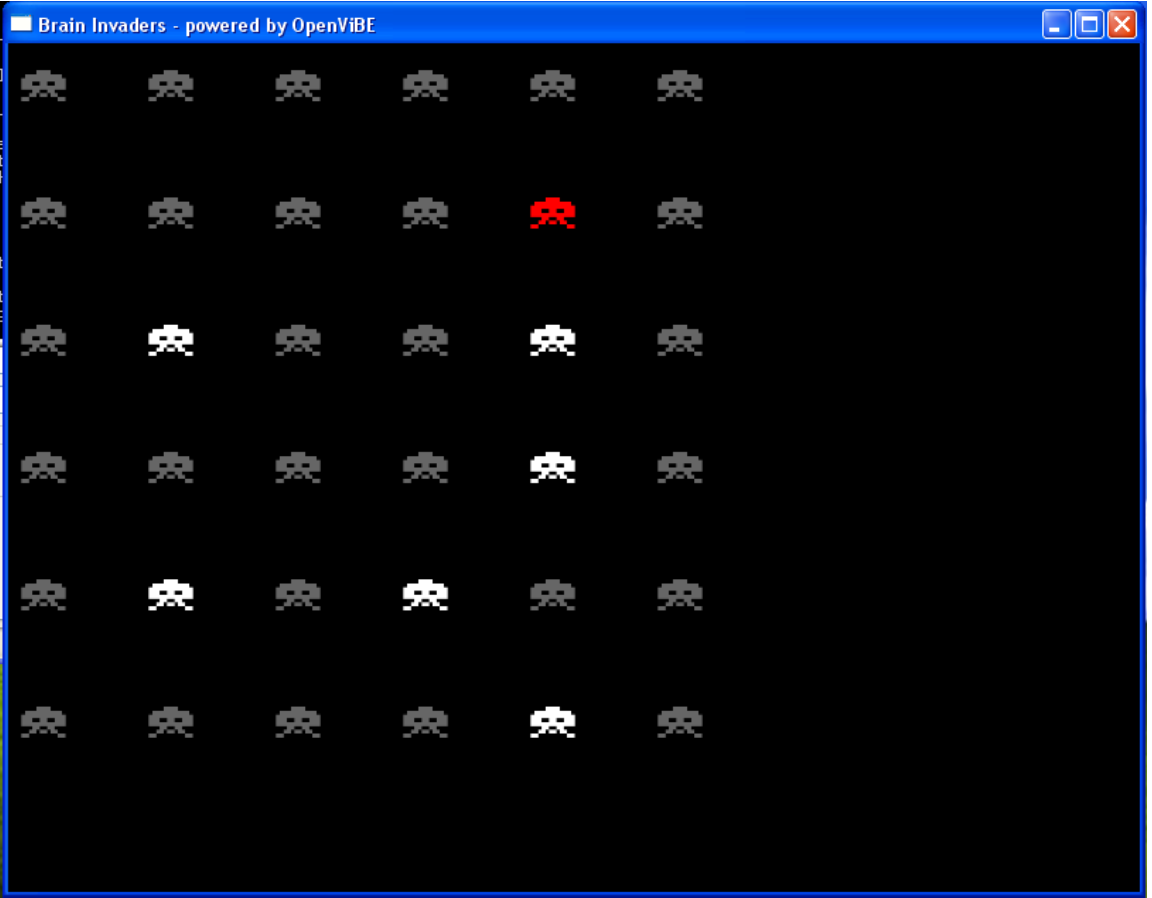
\includegraphics[width=0.65\textwidth]{figures/BrainInvaders15a.png}   
    %
    
    %\caption{SMC Learning Algorithm}
    \caption{Brain Invaders user interface at the game's introductory stage \cite{brainInvaders15a}}
    \label{fig: BrainInvaders}
    
    
\end{figure*}

\item \textbf{COGBCI} \cite{cogbci}: The COG-BCI dataset described in this study consists of recordings from 29 participants who completed three separate sessions, each conducted at an interval of 7 days. Each session included four distinct tasks: the Psychomotor Vigilance Task (PVT) \cite{dinges1985microcomputer}, the N-Back Task \cite{kirchner1958age}, the Multi-Attribute Task Battery (MATB) Task \cite{santiago2011multi}, and the Flanker Task \cite{eriksen1974effects}. These tasks were specifically designed to elicit various cognitive states. The authors employed a 64-electrode Ag-AgCl ActiCap (Brain Products Gmbh) EEG system with an ActiCHamp (Brain Products Gmbh) amplifier placed following the extended 10-20 system.  

%The COG-BCI database presented here is comprised of the recordings of 29 participants over 3 individual sessions with 4 different tasks namely Psychomotor Vigilance Task (PVT) \cite{dinges1985microcomputer}, N-Back Task \cite{kirchner1958age}, Multi-Attribute Task Battery (MATB) Task \cite{santiago2011multi} and Flanker Task \cite{eriksen1974effects} , designed to elicit different cognitive states. The measuring equipment used in this experimental campaign was an EEG system (electroencephalography) with 64 active Ag-AgCl electrodes (ActiCap, Brain Products Gmbh) and an ActiCHamp amplifier (Brain Products, Gmbh) positioned according to the extended 10-20 system. Data were sampled at 500 Hz. 
\smallskip

Due to its similarity to ERP paradigms, the Flanker task was selected as the optimal choice for our investigation out of all four tasks. The task induces interference and conflict effects, similar to the N400 paradigm, by presenting stimuli with congruent and incongruent flankers. As our study concentrates on ERP analysis, the flanker task provides a relevant framework for investigating cognitive control and neural responses using ERPs. The Flanker task is a choice reaction task derived from the study conducted by Eriksen and Eriksen (1974) \cite{eriksen1974effects} and is designed to induce conflict while making a binary choice. The participants are exposed to stimuli consisting of five arrows positioned at the center of a computer screen. Participants are instructed to respond to the central arrow while disregarding the surrounding (flanker) arrows. These flanker stimuli can aim in the same direction as the central target (congruent condition) or in the opposite direction (incongruent condition). The experimental procedure for the flanker task is illustrated in Figure \ref{fig:COGBCI}. Upon the conclusion of the trial, the participant is provided with feedback regarding the outcome of their performance, specifically indicating whether their response was correct, incorrect, or a miss. A total of 120 trials are conducted, with each complete run having an approximate duration of 10 minutes.   

\begin{figure*}
    %
     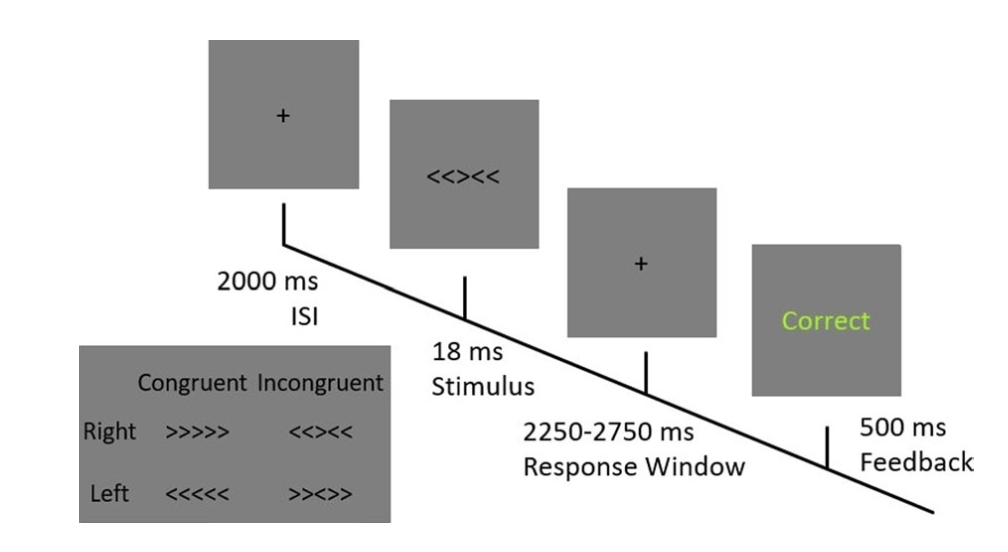
\includegraphics[width=0.90\textwidth]{figures/COGBCI.png}  
    %
    
    %\caption{SMC Learning Algorithm}
    \centering
    \caption{Flanker Task: After an Inter stimulus of 2000 ms, one of four possible stimuli (bottom left) is displayed for 18 ms. Participants then have between 2250 and 2750 milliseconds to respond before receiving 500 milliseconds of feedback \cite{cogbci}}
    \label{fig:COGBCI}
    
\end{figure*}


\item \textbf{ERPCORE: N400} \cite{hodapp2021n400}: 
This dataset has been used in various brainwave-based recognition studies such as \cite{arias2023performance, fallahi2023brainnet, ma2023n400}. It was developed for seven often studied ERP components: N170, MMN, N2pc, N400, P3, lateralized readiness potential (LRP), and ERN. The study included 40 participants, consisting of 25 females and 15 males. The participants were selected from the University of California, Davis community. The mean age of the participants was 21.5 years, with a standard deviation of 2.87. The age range of the participants was between 18 and 30 years. For our study, we focused on the N400 task. A word pair judgment task was employed to elicit the N400 component in this task. Every experimental trial comprised a red prime word that was subsequently followed by a green target word. Participants were required to indicate whether the target word was semantically related or unrelated to the prime word. The experimental setup for ERPCORE: N400 is depicted in Figure \ref{fig:ERPCORE}.   



\begin{figure*}
    %
    \centering
     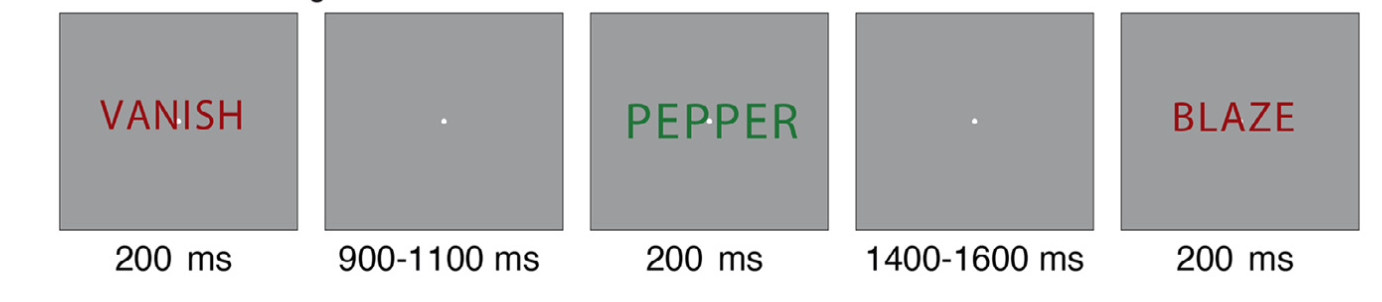
\includegraphics[width=\textwidth]{figures/ERPCORE.png}  
    %
    
    %\caption{SMC Learning Algorithm}
    \caption{The experimental setup for the ERPCORE: N400 task involving a specific configuration designed to elicit and measure the N400 component. \cite{erpcore}}
    \label{fig:ERPCORE}
    
    
\end{figure*}

\item \textbf{Mantegna et al. (mantegna)} \cite{mantegna2019distinguishing}: The dataset utilized in this study is derived from EEG investigations, specifically focusing on the analysis of N400 target word modulations. The researchers of this study examined the potential for disentangling integration and prediction in the modulation of Event-Related Potentials (ERPs) N400 during language processing. To do this, they used a stimulus assignment to complete sentences with rhyming words in various contexts with varying degrees of word predictability. All individuals who took part in the experiment were native speakers of the Dutch language, as the investigation was carried out in Dutch. In this experimental study, participants were provided with rhyming sentence completions. This experiment was carried out in three distinct stages. The first two stages consist of conducting online experiments with thirty and, respectively, 44 individuals. The third and ultimate stage of the study entails conducting an EEG experiment involving 31 participants. This experiment involves participants listening to a total of 135 sentences that rhyme, with either congruent or incongruent endings. The primary objective of this experiment is to elicit N400 ERPs. Figure \ref{fig: Mantegna} illustrates an instance of a sentence pair. 

%This dataset is based on EEG studies computing N400 target word modulations. The authors of this experiment investigated the possibility of separating integration from prediction in ERP N400 modulation accounts in language processing. To do so, they employed rhyming sentence completions as the stimulus task, across conditions that varied in word predictability. All the participants involved in the experiment were native Dutch speakers since the experiment was conducted in the Dutch language. In this experiment, rhyming sentence
%completions were given to participants. The experiment was conducted in three phases. The first two phases involve online experiments on thirty and 44 participants, respectively. The third and final phase is an EEG experiment, which involved listening to 135 rhyming sentences having congruent or incongruent endings, to elicit N400 ERP potentials. An example of sentence pair is depicted in figure 4.4. 
\begin{figure*}
    %
    \centering
     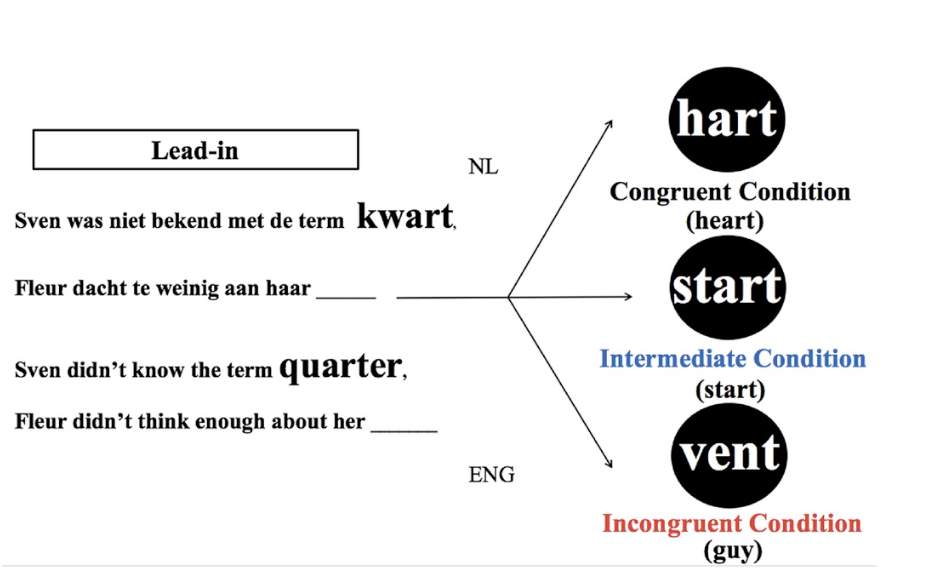
\includegraphics[width=0.80\textwidth]{figures/Mantegna.png}  
    %
    
    %\caption{SMC Learning Algorithm}
    \caption{Three alternative target words were selected for each sentence pair. In the congruent case, there was overlap in the rhymes, and the target word was easy to guess based on its meaning. In the middle case, there were words that rhymed with the target word, but the target word was not predictable based on its meaning. There was no rhyme overlap in the incongruent case \cite{mantegna2019distinguishing}}
    \label{fig: Mantegna}
    
    
\end{figure*}

\end{enumerate}
Once the datasets have been collected, the next step is to create an outline of the benchmarking, which is covered in the following section.  

\section{Workflow}
\label{sec:Solution Approach:Workflow}

Our benchmarking framework is organized into five modules: datasets, paradigm, evaluation, pipeline, and analysis. The next section contains detailed information on all of the modules described above. We also provide statistical and visualization tools to help visualize the performance of authentication techniques.
\begin{itemize}

\item \textbf{Datasets}: This module offers abstract access to open datasets.  It entails downloading open datasets from the internet and providing effective data management. 

\item \textbf{Paradigm}: The purpose of this module is to conduct pre-processing on the unprocessed EEG data. Datasets exhibit distinct characteristics based on ERP paradigms such as P300 and N400. Nevertheless, both conditions elicit ERP responses after  the individual's exposure to unexpected stimuli. Consequently, the datasets for the P300 and N400 paradigms undergo pre-processing using identical parameters. 

%This module is made to perform pre-processing on the raw EEG data. Datasets are differentiated by ERP paradigms like P300 and N400. However, both elicit ERP responses after the person is exposed to unexcepted to stimuli. As a result, the pre-processing is done on the datasets for P300 and N400 paradigm with the same parameters. 

\item \textbf{Pipeline}: This module extracts features from data that has been pre-processed. These characteristics are extracted in the time and frequency domains and are discussed in detail in chapter 5.3.   

\item \textbf{Evaluation}:  The authentication algorithms are developed and utilized for training and testing the features extracted within the pipeline module. The performance of authentication modules is assessed through various evaluation schemes, including within-session and cross-session evaluation. In addition, we will evaluate the efficacy of authentication protocols across multiple threat scenarios, including both closed-set and open-set scenarios. 

\item \textbf{Analysis}: After obtaining the performance metrics, this module offers various methods for conducting statistical analysis on the performance of diverse datasets and algorithms. The analysis will be conducted utilizing multiple visualization techniques.
\end{itemize}

It is important to acknowledge that the execution of the procedures above necessitates the utilization of the Scikit-Learn \cite{Scikit_Learn} pipeline. This pipeline facilitates the execution of various python pipelines comprising distinct datasets, paradigms, feature extraction methods, and algorithms. 

\begin{figure*}
    %
    \centering
     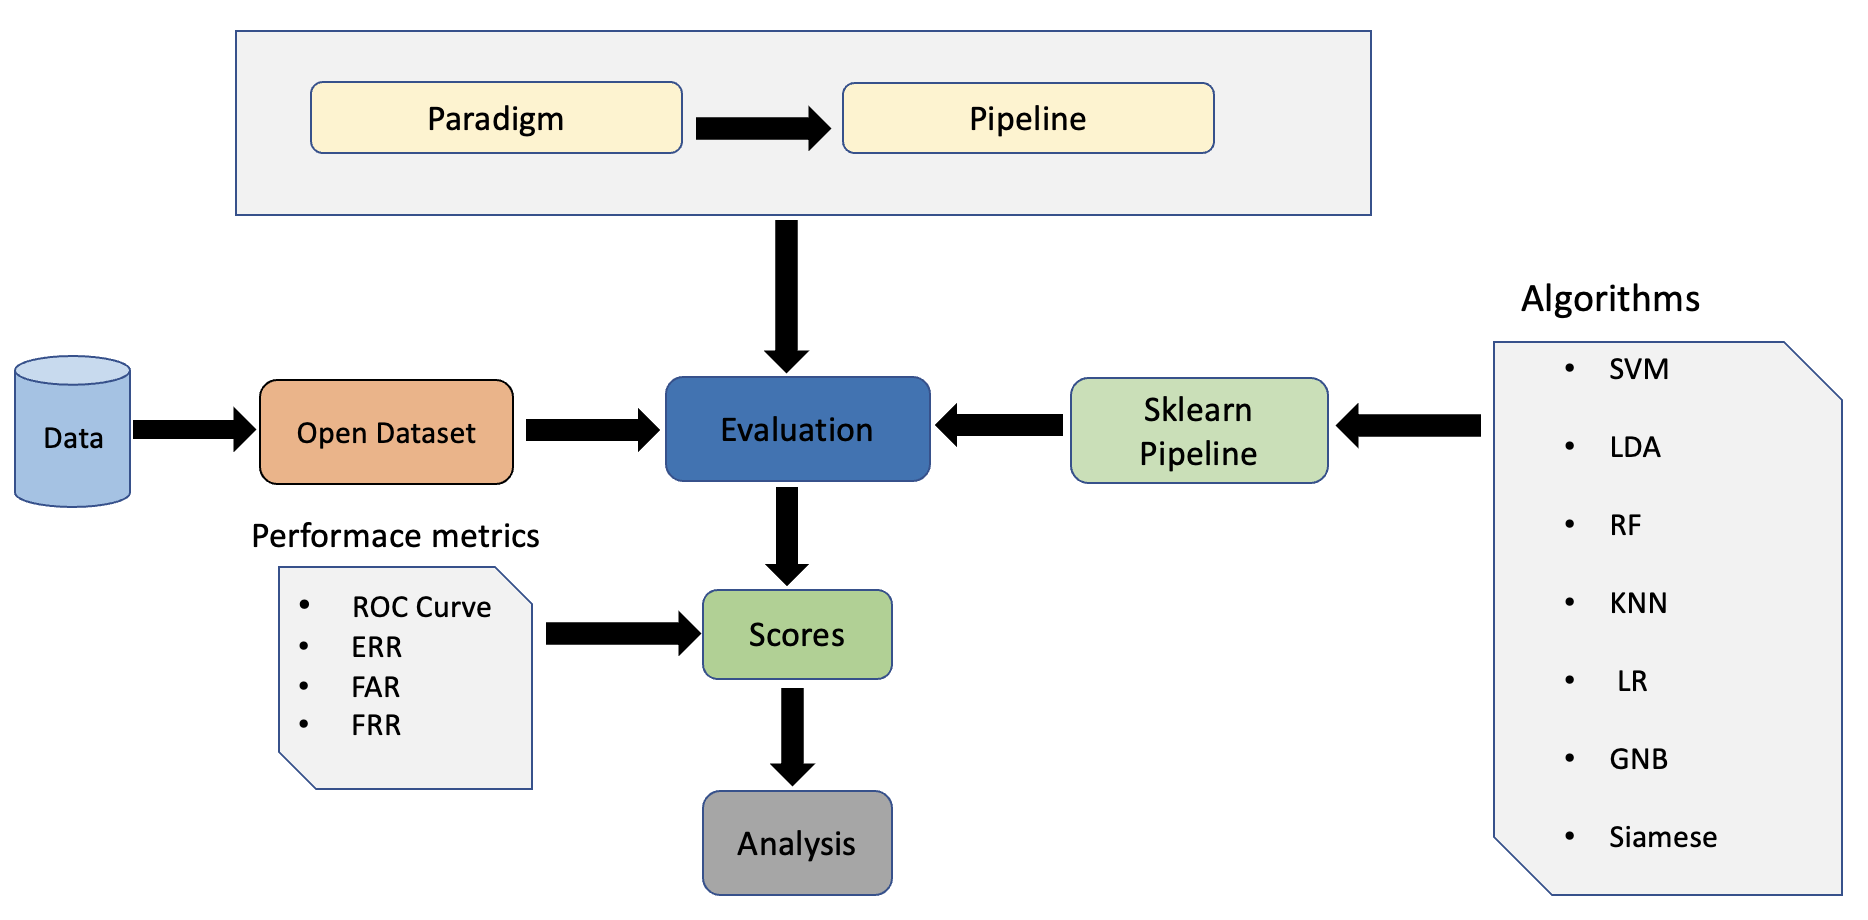
\includegraphics[width=0.90\textwidth]{figures/Architecture/Updated_Architecture.png}  
    %
    
    %\caption{SMC Learning Algorithm}
    \caption{Overview of benchmarking suite}
    \label{fig:Benchmarking suite}
    
    
\end{figure*}

